\chapter{Results}
\label{results}

\begin{figure*}
    \centering
    \begin{subfigure}{\linewidth}
        \centering
           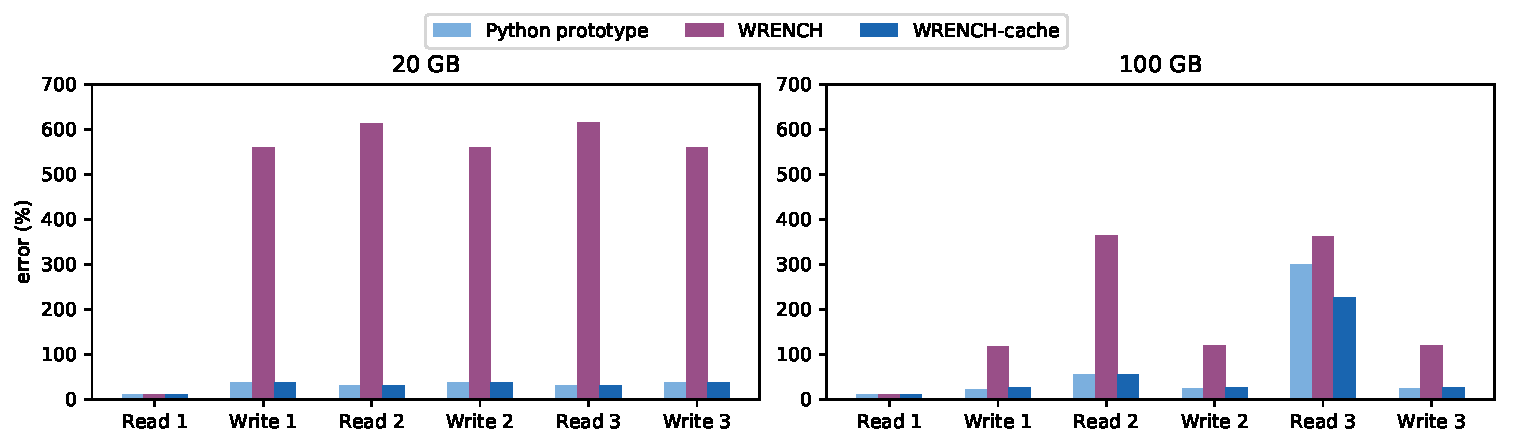
\includegraphics[width=\linewidth]{result/single/figures/single_errors.pdf}
           \vspace*{-0.7cm}
           \caption{Absolute relative simulation errors}
           \vspace*{0.5cm}
           \label{fig:single_error}
        \end{subfigure}
    \begin{subfigure}{\linewidth}
        \centering
        %    Gray shades represent task phases (read, compute and write).
        %    Lines represent memory usage along pipeline execution time.}
           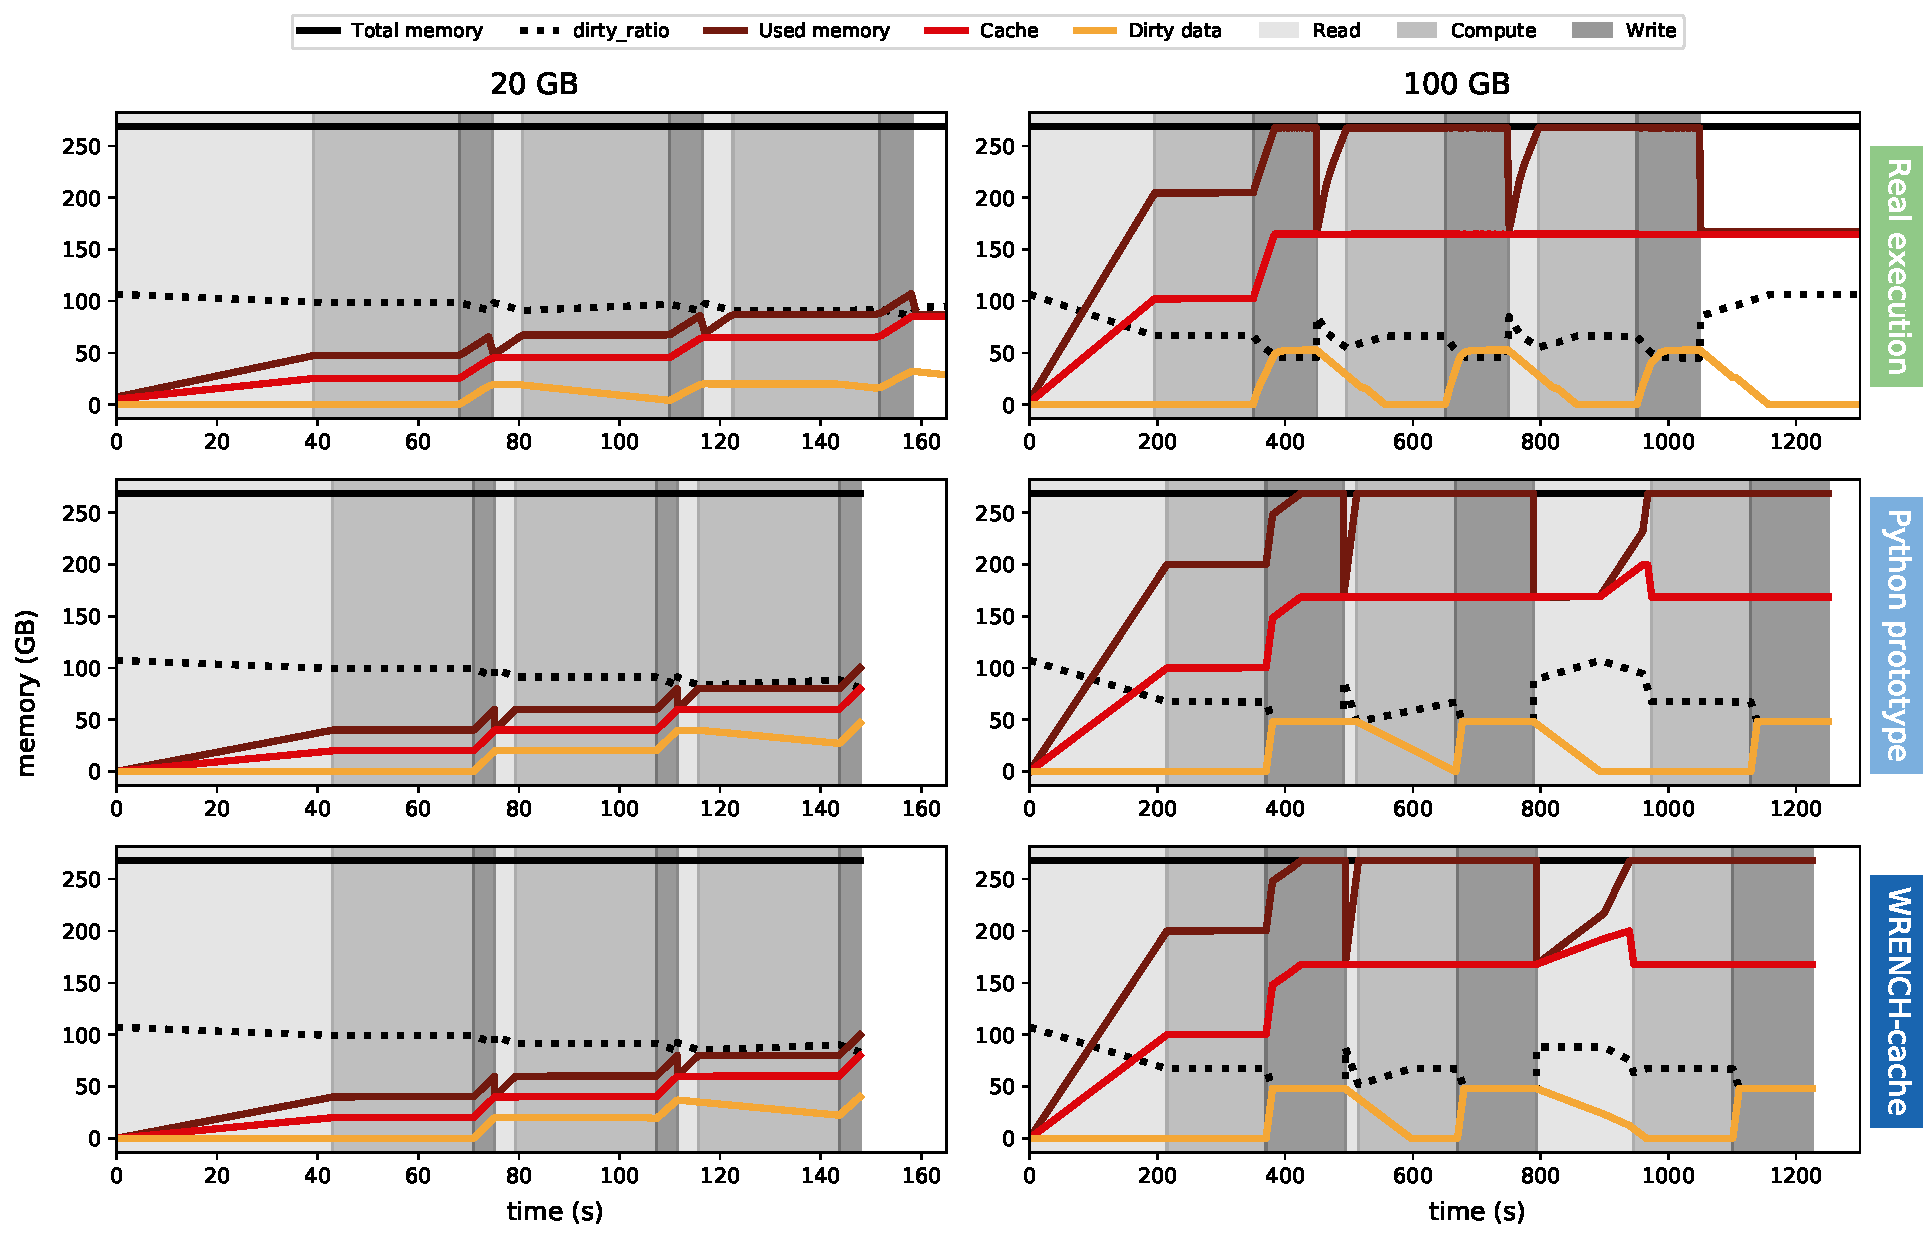
\includegraphics[width=\linewidth]{result/single/figures/single_memprof.pdf}
           \vspace*{-0.7cm}
           \caption{Memory profiles}
           \vspace*{0.5cm}
           \label{fig:single_memprof}
    \end{subfigure}
    \begin{subfigure}{\linewidth}
        \centering
           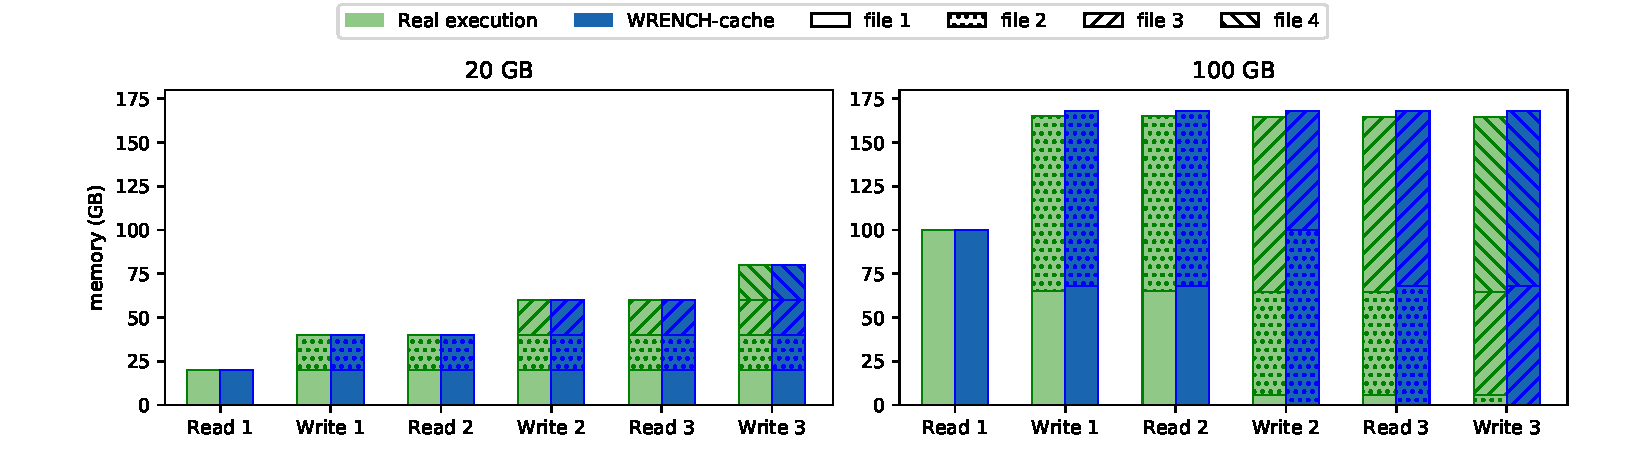
\includegraphics[width=1.05\linewidth]{result/single/figures/cached_files.pdf}
           \caption{Cache contents \emph{after} application I/O operations}
        %    \textcolor{red}{Update real results of 20GB}}
           \label{fig:single_cache}
    \end{subfigure}
    \caption{Single-threaded results (\textit{Exp 1})}
\end{figure*}

\section{Single-threaded execution (Exp 1)}

The page cache simulation model drastically reduced I/O simulation
errors in each application task (Figure~\ref{fig:single_error}). The first read was not impacted
as it only involved uncached data. Errors were reduced from an average
of 345\% in the original \wrench to 46\% in the Python prototype and
39\% in \wrench-cache. Unsurprisingly, the original \wrench simulator
significantly overestimated read and write times, due to the lack
of page cache simulation. Results with files of 50~GB and 75~GB
showed similar behaviors and are not reported for brevity.

\wrench simulation errors were substantially lower with 100~GB
files than with 20~GB files, due to the fact that part of the
100~GB file needed to be read and written to disk, the only storage
device in \wrench, as it did not fit in cache. Conversely,
simulation errors of the Python prototype and \wrench-cache were higher with
100~GB files than with 20~GB files, due to idiosyncrasies in the kernel
flushing and eviction strategies that could not be easily modeled.

Simulated memory profiles were highly consistent with the real ones
(Figure~\ref{fig:single_memprof}). With 20~GB files, memory profiles almost exactly matched the
real ones, although dirty data seemed to be flushing faster in real
life than in simulation, a behavior also
observed with 100~GB files. With 100~GB files, used memory reached
total memory during the first write, triggering dirty data
flushing, and droped back to cached memory when application tasks
released anonymous memory. Simulated cached memory was highly
consistent with real values, except toward the end of Read 3 where
it slightly increased in simulation but not in reality. This
occurred due to the fact that after Write 2, File 3 was only partially
cached in simulation whereas it was entirely cached in the real
system. In all cases, dirty data remained under the dirty ratio as
expected. The Python prototype and \wrench-cache exhibited nearly
identical memory profiles, which reinforces the confidence in our
implementations.

The content of the simulated memory cache was also highly
consistent with reality (Figure~\ref{fig:single_cache}). With 20~GB
files, the simulated cache content exactly matched reality, since
all files fitted in page cache. With 100~GB files, a slight
discrepancy was observed after Write 2, which explains the
simulation error previously mentioned in Read 3. In the real
execution indeed, File 3 was entirely cached after Write 2, whereas
in the simulated execution, only a part of it was cached. This was
due to the fact that the Linux kernel tends to not evict pages that
belong to files being currently written (File 3 in this case),
which we could not easily reproduce in our model.

\begin{figure*}
    \begin{subfigure}{\linewidth}
        \centering
        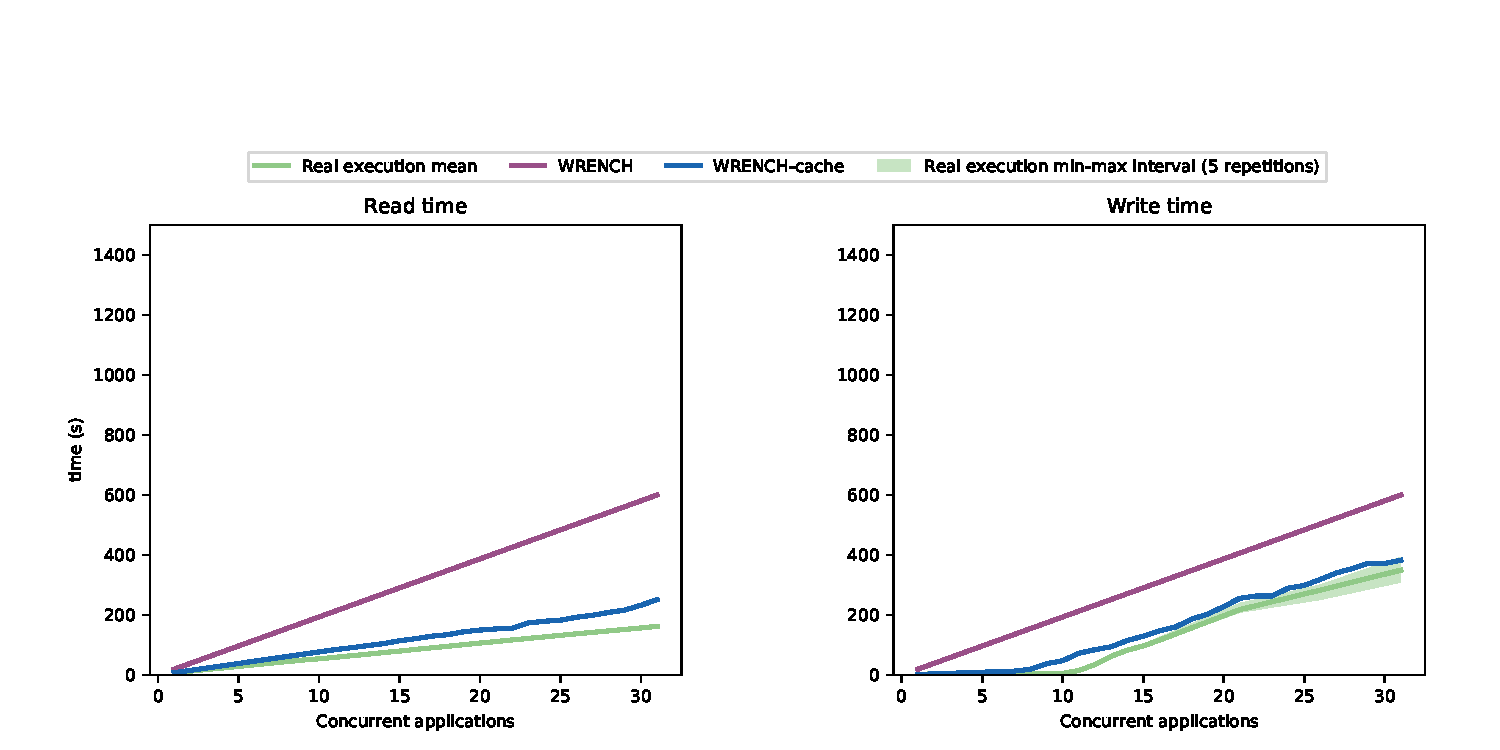
\includegraphics[width=\linewidth]{result/multi/figures/multi_local.pdf}
    \end{subfigure}
    \caption{Concurrent results with 3~GB files (\textit{Exp 2})}
    \label{fig:multi_local}
\end{figure*}

\section{Concurrent applications (Exp 2)}

The page cache model notably reduced \wrench's simulation error
for concurrent applications executed with local I/Os
(Figure~\ref{fig:multi_local}). For reads, \wrench-cache
slightly overestimated runtime, due to the discrepancy between
simulated and real read bandwidths mentioned before. 
For writes, \wrench-cache
retrieved a plateau similar to the one observed in the real
execution, marking the limit beyond which the page cache was
saturated with dirty data and needed flushing.

\begin{figure}[b]
    \begin{subfigure}{0.95\linewidth}
        \centering
        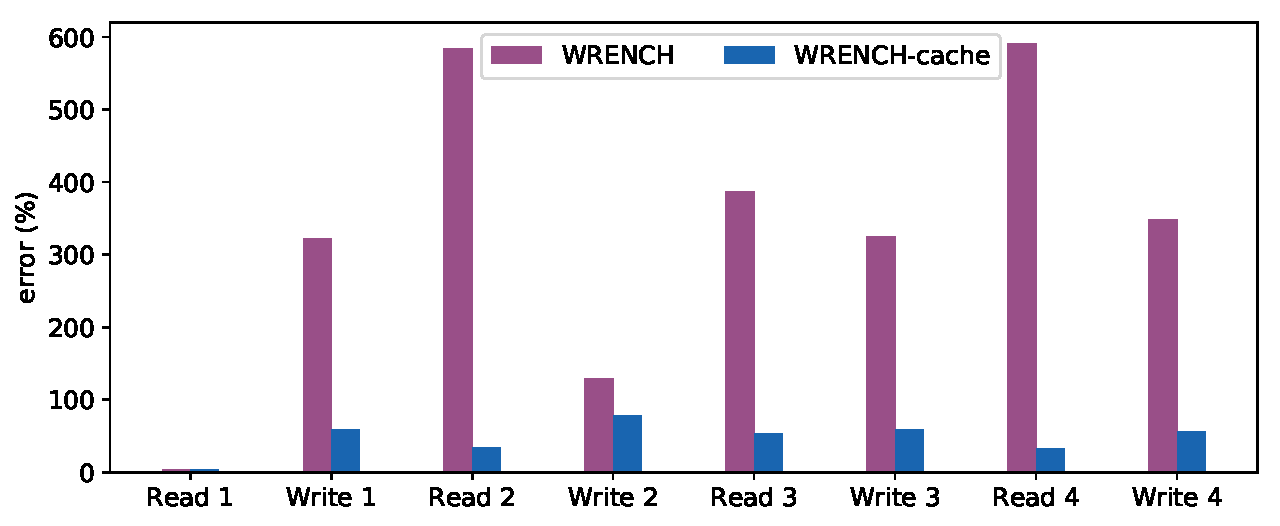
\includegraphics[width=\linewidth]{result/nighres/figures/nighres_errors.pdf}
    \end{subfigure}
    \caption{Real application results (\textit{Exp 4})}
    \label{fig:nighres}
\end{figure}

\section{Remote storage (Exp 3)}

Page cache simulation importantly reduced simulation error
on NFS storage as well (Figure~\ref{fig:multi_nfs}). This
manifested only for reads, as the NFS server used writethrough rather than writeback cache.
Both \wrench and \wrench-cache
underestimated write times due to the discrepancy between
simulated and real bandwidths mentioned previously. For reads,
this discrepancy only impacted the results beyond 22
applications since before this threshold, most reads resulted in cache
hits.


\section{Real application (Exp 4)}
Similar to the synthetic application, simulation errors were
substantially reduced by the WRENCH-cache simulator compared to
WRENCH (Figure~\ref{fig:nighres}). On average, errors were reduced
from 337~\% in WRENCH to 47~\% in WRENCH-cache. 
The first read happened entirely from disk and was therefore 
very accurately simulated by both WRENCH and WRENCH-cache.

\begin{figure*}
    \begin{subfigure}{\linewidth}
        \centering
        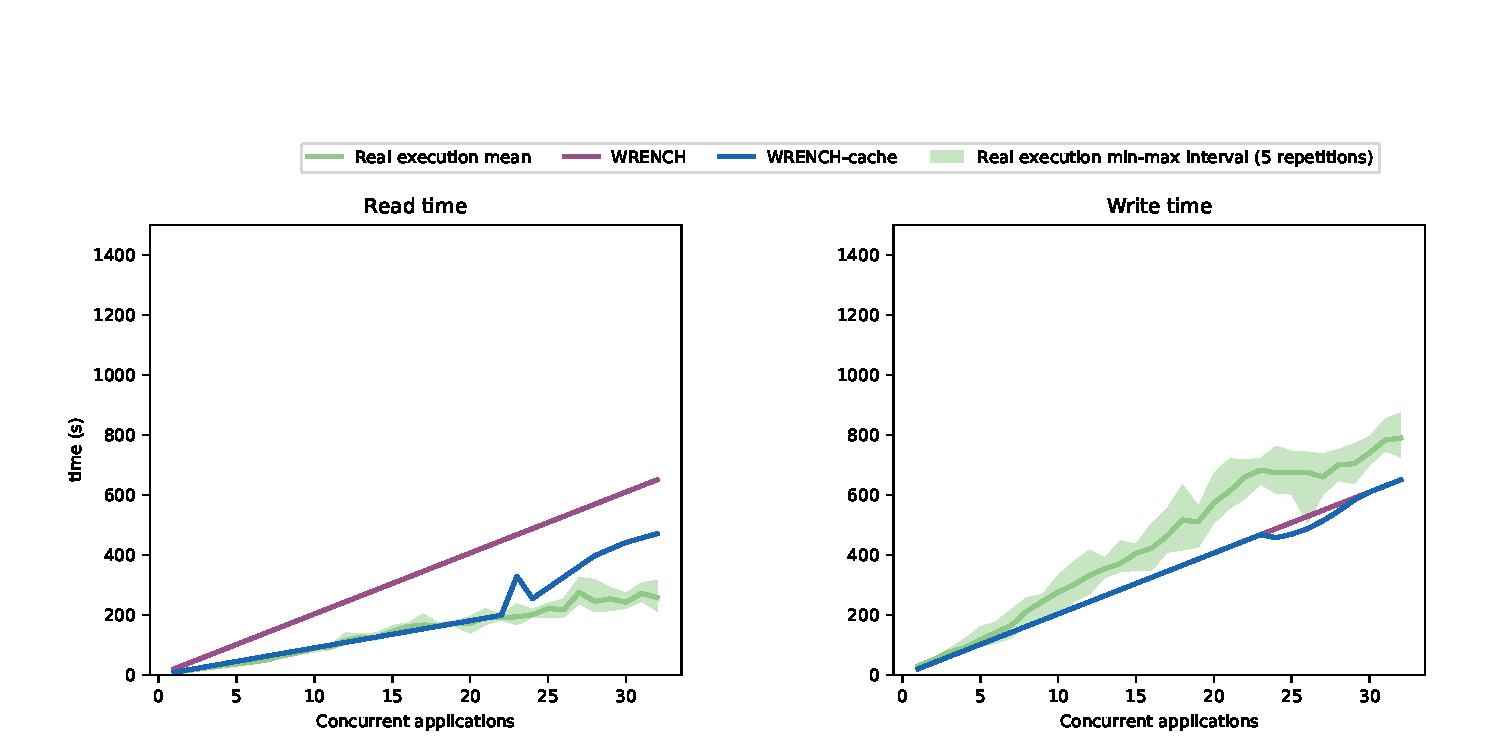
\includegraphics[width=\linewidth]{result/multi/figures/multi_nfs.pdf}
    \end{subfigure}
    \caption{NFS results with 3~GB files (\textit{Exp 3})}
    \label{fig:multi_nfs}
\end{figure*}

\begin{figure}
    \begin{subfigure}{\columnwidth}
        \centering
        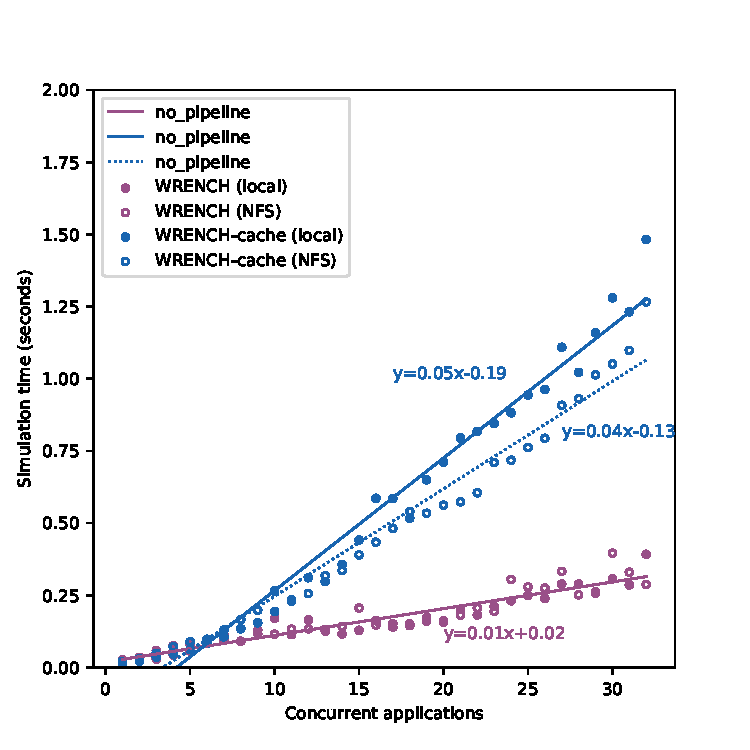
\includegraphics[width=\linewidth]{result/multi/figures/simulation_time.pdf}
    \end{subfigure}
    \caption{Simulation time comparison. \wrench-cache scales
    linearly with the number of concurrent applications, albeit
    with a higher overhead than \wrench.}
    \label{fig:multi_time}
\end{figure}

\section{Simulation time}
As is the case for \wrench, simulation time with \wrench-cache scales
linearly with the number of concurrent applications
(Figure~\ref{fig:multi_time}, p \textless $10^{-24}$). However, the page
cache model substantially increases simulation time by
application, as can be seen by comparing regression slopes in
Figure~\ref{fig:multi_time}. Interestingly, \wrench-cache is faster with 
NFS I/Os than with local I/Os, most likely due to the use of writethrough
cache in NFS, which bypasses flushing operations.